\documentclass[DIV=12,headings=normal,pdftex,headinclude=false,footinclude=false,final]{scrreprt}
\usepackage{spreadtab}
\usepackage{xspace}
\usepackage[ngerman]{babel}
\usepackage{tocbasic}
\usepackage{graphicx}
\usepackage[linkcolor=black,colorlinks=true,urlcolor=blue]{hyperref}
%\usepackage{abntcite}
\usepackage{scrlayer-scrpage}
\usepackage{longtable}
\usepackage{caption}
\usepackage{float}
\usepackage{xcolor}
\usepackage{colortbl}
\usepackage[utf8]{inputenc}
\usepackage[T1]{fontenc}
\usepackage{wrapfig}

\usepackage{listings}
\usepackage{xcolor}

\usepackage{helvet}
%\usepackage[nohyperlinks, printonlyused, withpage, smaller]{acronym}
%\usepackage[backend=biber,style=numeric,citestyle=numeric]{biblatex}
%\usepackage{csquotes}

%\addbibresource{itsec.bib}



\definecolor{codegreen}{rgb}{0,0.6,0}
\definecolor{codegray}{rgb}{0.5,0.5,0.5}
\definecolor{codepurple}{rgb}{0.58,0,0.82}
\definecolor{backcolour}{rgb}{0.96,0.96,0.96}

\lstdefinestyle{mystyle}{
    backgroundcolor=\color{backcolour},   
    commentstyle=\color{codegreen},
    keywordstyle=\color{blue},
    numberstyle=\tiny\color{codegray},
    stringstyle=\color{codepurple},
    basicstyle=\ttfamily\footnotesize,
    breakatwhitespace=false,         
    breaklines=true,                 
    captionpos=b,                    
    keepspaces=true,                 
    numbers=left,                    
    numbersep=5pt,                  
    showspaces=false,                
    showstringspaces=false,
    showtabs=false,                  
    tabsize=2
}
\lstset{style=mystyle}


\graphicspath{{./}{./Images/}}

\setlength\headheight{1.75cm}
\ihead{\small{G. Hauschild, K. Wilfert StuArb IT-Security 2020/21}}
\chead{}
\ohead{
\includegraphics[height=0.05\textheight]{fh_logo}}
\pagestyle{scrheadings}


\titlehead{
\includegraphics[width=5cm]{fh_logo}}
\title{Studienarbeit über die Schwachstelle\\CVE-2017-0144\\''EternalBlue''}
\subtitle{IT-Sicherheit\\Wintersemester 2020/2021}
\author{Georg Hauschild (00175118) und Kay Wilfert (01642116)}
\date{\today \\
Im Rahmen der Wahlkurses IT-Sicherheit wurde die Sicherheitlücke, welche im März 2017 mit dem Beinamen
EternalBlue bekannt wurde, auf ihre inneren Vorgänge untersucht.
Von der NSA für verdeckte Ermittlungen benutzt, stellte Sie für viele Windows-Versionen
aufgrund der dort integrierten SMBv1 Schnittstelle eine Bedrohung dar. Es wird näher untersucht,
welche Bugs ausgenutzt werden, um über das SMB-Protokoll eine Remote Code Execution zu bewirken.
}


\begin{document}
\maketitle

\pagenumbering{roman}

\tableofcontents

\listoffigures

\chapter*{Abkürzungsverzeichnis}

\noindent
\textbf{CIFS}: Common Internet File System\\
Urversion des SMB, Begriff in frühen Versionen austauschbar\\

\noindent
\textbf{CVE}: Common Vulnerabilities and Exposures\\
Liste von Schwachstellen und Sicherheitslücken, jede eindeutig mittels eines CVE-Codes identifizierbar\\

\noindent
\textbf{FEA}: File Extension Attributes\\
Dateisystemfunktion für nicht weiter interpretierte Metadaten von Dateien\\

\noindent
\textbf{MBR}: Master Boot Record\\
Enthält notwendiges Startprogramm für verschiedene OS, sowie Partitionstabelle.\\

\noindent
\textbf{MFT}: Master File Table\\
Master File Table, enthält Informationen über abgelegte Dateien auf NTFS Datenträgern\\

\noindent
\textbf{NAS(-Server)} Network Accessible Storage (Server)\\
Im lokalen Netzwerk erreichbarer Server, der Dateien und Verzeichnisse für Teilnehmer zur Verfügung stellt

\noindent
\textbf{RCE}: Remote Code Execution\\
Eine Attacke, bei der Angreifer Schadcode auf entfernten Rechnern ausführen\\

\noindent
\textbf{SMB(v1)}: Server Message Block (Version 1)\\
Netzwerkprotokoll zum Austausch von Dateien und Services im Netzwerk\\

\noindent
\textbf{TCP}: Transmission Control Protocol\\
Protokoll zum Datenaustausch im Netzwerk über aufgebaute Verbindung\\

\noindent
\textbf{UDP}: User Datagram Protocol\\
Protokoll zur Datenübermittlung ohne zuvor aufgebaute Verbindung\\


\newpage
\pagenumbering{arabic}

%\chapter{Kurzzusammenfassung}



\chapter{Malware auf EternalBlue Basis}
In vielerlei Hinsicht ist die Entstehungsgeschichte des EternalBlue Exploits eng mit der US-amerikanischen National Security Agency verbunden. Eine Unterabteilung der Agency, zum damaligen Zeitpunkt als "Tailored Access Operations" bekannt \cite{CS}, untersuchte über ein Jahr lang das Windows Betriebssystem auf Schwächen, die der Agency beim Zugriff auf fremde Systeme helfen könnten\cite{WP}. Letzten Endes wurden mehrere Sicherheitslücken im SMB Protokoll der Windows Plattform gefunden, die es ermöglichen, mittels eines speziell angefertigten Paketes einen Rechner zu kapern und auf ihm beliebigen Code auszuführen \cite{Avast}.
Eigens für die Sicherheitslücke, die später als CVE-2017-0144 veröffentlicht wurde, programmierte die Agency das Hacking-Tool EternalBlue, so benannt nach der Tendenz, die angegriffenen Rechner zu crashen, was einen bluescreen zu folge hatte. Das Hacking Tool zählte intern zur NOBUS-Gruppe (Nobody but us), da eine solche Sicherheitslücke aufgrund der enormen Konsequenzen nie an die Öffentlichkeit gelangen sollte \cite{CS}. Dieses Vorgehen, Zero-Day-Exploits zu sammeln und zu Waffen umzufunktionieren sorgte schon damals in einigen NSA Officials für Unbehagen, was, wie sich herausstellte, eine berechtigte Kritik war \cite{WP}.
Jedoch kam es genau zu einem solchen Ernstfall, als die Hackergruppe der “Shadow Brokers” im August 2016 die gesamte Familie der SMB-Schwachstellen zusammen mit dem Hacking Tool veröffentlichte. Somit waren auch Amateure fähig, die Lücke zu nutzen, um Schaden anzurichten. Die NSA reagierte zunächst lediglich mit einer Benachrichtigung an Microsoft, klärte allerdings den generellen Populus nicht bezüglich der enormen Gefahr, die von dem Leak ausging, auf \cite{WP}.

\begin{figure}[H]
    \centering
    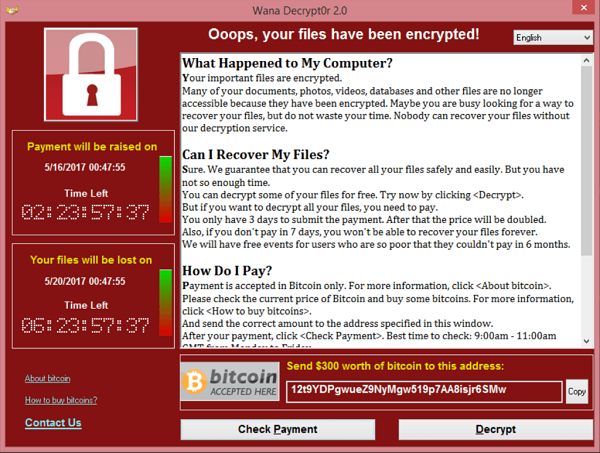
\includegraphics[width=10cm]{wanna_decrypt0r_2.0.png}
    \caption[WannaDecryptor Screenshot, URL: <https://securelist.com/   wannacry-ransomware-used-in-widespread-attacks-all-over-the-world/78351/>]{Ein Screenshot des  WannaDecryptor 2.0 Virus}
    \label{img:wanna_decrypt0r}
\end{figure}

\noindent
Am 12. Mai 2017 wurde das gewaltige Gefahrenpotenzial dann realisiert. Ein Ransomware-Virus namens WannaCrypt, auch bekannt unter einigen Aliasnamen, nutze den modifizierten EternalBlue Code zum Infizieren und Verschlüsseln von Windows-PCs auf der ganzen Welt \cite{Avast}. Zwar veröffentlichte Microsoft schon zwei Tage nach Ausbruch ein Sicherheitsupdate, was aber erst nach und nach von Nutzern installiert werden musste \cite{MSSB}. Deshalb wurden die persönlichen Daten unzähliger Nutzer auf deren Rechnern verschlüsselt und der Zugriff dauerhaft gesperrt. Zu sehen war wie bei jeder Ransomeware nur eine Lösegeldforderung und das Versprechen, die Daten durch eine Zahlung, zum Beispiel in Bitcoin, wieder herzustellen. Sonst würden die Daten gelöscht werden. Das Virus verbreitete sich mit einer Geschwindigkeit von circa 10.000 Neuinfektionen pro Stunde, sodass nach dem ersten Tag bereits 230.000 Windows-Maschinen in über 150 Ländern betroffen waren. Dabei schienen die Attacken wahllos verschiedene Ziele anzugreifen, wodurch keine spezifische Taktik erkennbar war. Es folgte ein enormer monetärer Schaden in der Höhe von ungefähr vier Milliarden US-Dollar, wobei ein genauer Betrag aufgrund der hohen Dunkelziffer schwer einzuschätzen und nicht bekannt ist, wie viele Personen auf die Drohung reagierten \cite{Avast}.

\begin{figure}[H]
    \centering
    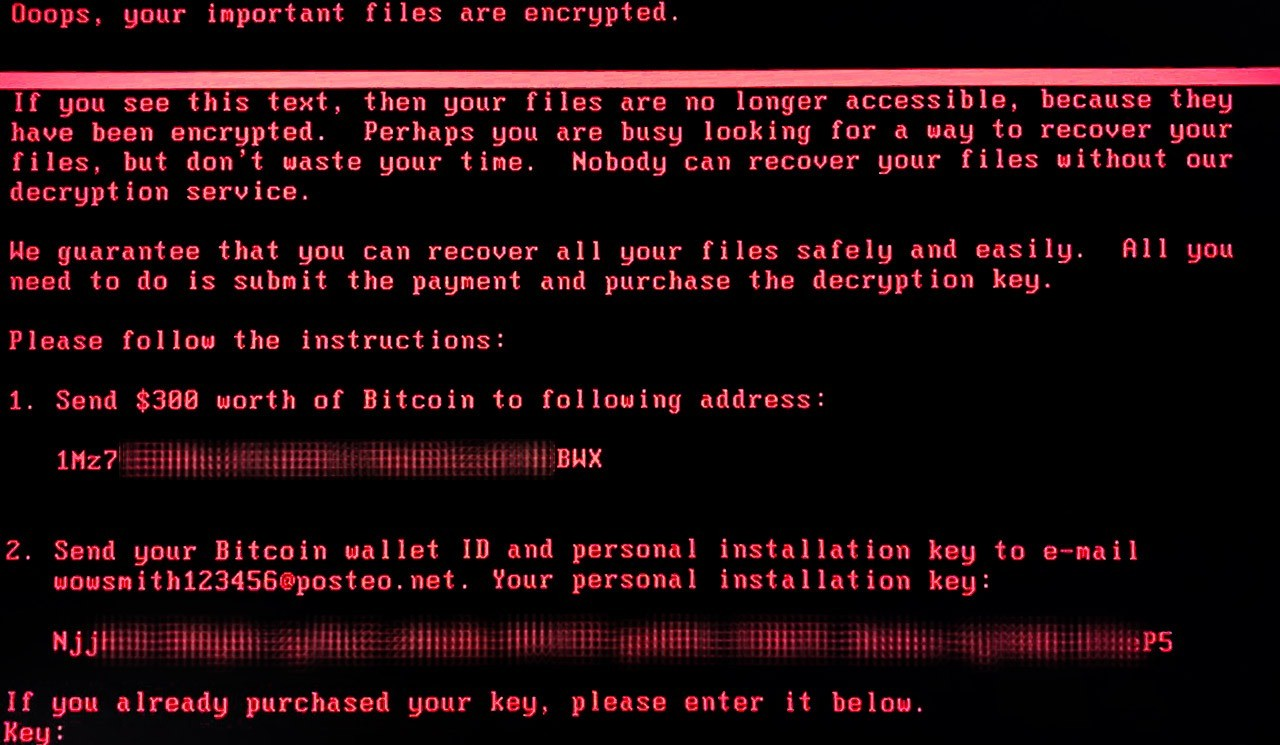
\includegraphics[width=10cm]{notpetya_ransomware.jpg}
    \caption[NotPetya Screenshot, Nutzer ''GrEat''/Kaspersky, URL: <https://media.kasperskydaily.com/wp-content/uploads/sites/92/2017/06/27133735/wannamore-ransomware-screenshot.jpg>]{Screenshot einer Variante des WannaCry Virus}
    \label{img:not_petya}
\end{figure}

\noindent
Als noch verheerender erwies sich der NotPetya Virus, eine mit dem EternalBlue-Kern aufgerüstete Version eines bereits im Vorjahr umgehenden, weniger bekannten und weitaus weniger schädlichen Virus am 16.6.2017. NotPetra zeichnete sich dadurch aus, dass sowohl MBR als auch MFT verschlüsselt worden sind, was eine Wiederherstellung der Daten unmöglich machte, auch wenn der Sperrbildschirm dies gegen 300 USD versprach. Der durch diese zweite gigantische Ransomware-Welle verursachte Schaden wurde auf etwa 10 Milliarden USD geschätzt, wobei der Datenverlust und die Menschenleben, die durch lahmgelegte Rechner in Krankenhäusern und öffentlichen Einrichtungen in Gefahr gebracht worden sind, nicht mit eingerechnet sind \cite{Avast}.\\
Wie sich nach Analyse der Malware heruasstellte besaß keiner der beiden Viren, insbesondere wie oben beschrieben NotPetya, die nötige Infrastruktur auf, um nach dem Zahlen des Lösegelds in Bitcoin das Entschlüsseln der Daten wieder zu ermöglichen. Das lässt darauf schließen, dass nicht monetäere Gewinn, sondern Schaden das Hauptziel der Hacker war \cite{Sil}.


\noindent
Microsoft reagiere im Angesicht des entstandenen Schadens und des Mangels an Vorsicht der US-Regierung mit einer Warnung, dass der Trend, Zero-Days zu sammeln, um Sie für digitale Kriegsführung zu nutzen ein gefährliches Unterfangen sei. Es wurde zu Verhandlungen für eine digitale Genfer Konvention aufgerufen und ein Entwurf vorgelegt, der einen groben Plan skizziere, keine Repertoire an Sicherheitlücken anzulegen und Cyberkriegsführung zu regulieren \cite{MS:EB}.

\chapter{Der EternalBlue Exploit}
Dieses Kapitel beleuchtet die inneren Vorgänge des Server Message Blocks 1.0 und die Fehler, die das erfolgreiche Ausführen eines RCE Angriffs auf Windows Hosts ermöglichen. Die National Vulnerability Database bewertete diese Sicherheitslücke in CVSS Version mit 8.1 von maximal 10 Punkten \cite{NVD} als schwerwiegend. Zweifelsohne aufgrund der sehr hohen Verbeitung der Verwundbarkeit und des Schweregrads eines Hacking-Angriffs. 

\section{Grundlagen}
Um den Exploit besser verstehen zu können, müssen vorab einige grundlegende Begriffe erklärt werden, die für die Durchführung einer solchen Hacking Attacke essenziell sind.

\section{Das SMB Protokoll}
Das im schon mehrere Dekaden alte Protokoll wurde von 1983 von Barry Feigenbaum (IBM) 1983 vorgestellt und fand später erstmals in Windows 95 Verwendung. Das in der damiligen Forrm als CIFS bekannte Protokoll dient seitdem auf jeder Windows Plattform bis heute dem Austausch über Netzwerkressourcen wie Dateien, Verzeichnisse, Drucker und Programmierschnittstellen \cite{CompWeek:SMB}. Spätere Server Message Block Iterationen wurden dann stets mit Versionsnummern versehen. Anfangs baute CIFS Verbindungen über ein weiteres Protokoll namens NetBIOS over TCP auf, das die UDP Ports 137 für Namensauflösung, 138 für Paketübermittlung und TCP-Port 139 für Verbindungsaufbau und Datenübertragung nutzte \cite{MS:NetBIOS}. Dieses wurde allerdings schon ab Windows 2000 von regulären TCP-Verbindungen auf Port 445 und dem DNS-Protokoll abgelöst \cite{IONOS}. Die davor meist als CIFS bezeichnete Urversion der unter Windows implementierten Schnittstelle wird von hier an im Rest der Arbeit als SMBv1 bezeichnet. Weiterhin wird es sich stets um die Version des Protokolls über TCP auf Port 445 handeln.\\
Trotz der engen Assoziation mit Windows handelt es sich jedoch um ein plattform- und dateiformatunabhängiges Protokoll, das via Samba Shareware auch auf Linux angewendet werden kann\cite{IONOS}. 

\section{Der non paged Pool}
Zur Verwaltung des Arbeitsspeicherressourcen besitzt Windows einen Memory Manager. Dieser hat als Aufgabe, für Prozesse und deren Verwaltung Arbeitsspeicher zu reservieren und wieder danach wieder frei zu geben. Der Memory Manager schöpft bei dieser Verwaltung Speicherbereiche aus dem für das System reservierten Arbeitsspeicher, der bereits für den virtuellen Adressraum gemappt wurde. Unterteilt wird hierbei in zwei sogenannte Memory Pools, in denen Memoryblöcke allokiert werden: Den paged und den non-paged Memory Pool \cite{MS:MemPools}. Die zusätzliche Abstraktionschicht des Mappens von virtuellen auf physikalische Speicheradressen ermöglicht unter anderem dieses Paging. Als Paging bezeichnet man hierbei das Ein- und Auslagern von Arbeitsspeicherblöcken ins Dateisystem, um in Ausnahmefällen mehr Speicher zur Verfügung zu haben als physikalisch verbaut \cite{CompWeek:Paging}.\\
Der non-paged Memory Pool ist für den EternalBlue Exploit relevant, da in ihm durch mehrere Bugs im SMB-Protokoll Speicherbereiche reserviert, frei gegeben und gelesen werden, die zum Laden des Schadcodes dienen.

\section{File Extended Attributes}
File Extended Attributes sind Datenstrukturen, die erweiterte Metadaten beherbergen, die nicht für das System notwendig sind. Darin können zum Beispiel der Autor, das Encoding einer Textdatei oder andere Informationen gespeichert werden \cite{Wiki:FEA}. Solche zusätzlichen Informationen werden im SMBv1 Protokoll in FEA Strukturen gespeichert, die die Form von Key-Value-Paaren annehmen, welche wiederum in Listen abgespeichert werden \cite{CP}. SMB ist ein plattformübergreifendes Protokoll, welches demnach auch für mehrere Dateisysteme besagte Listenstrukturen implementiert haben muss. Darunter fällt auch das OS/2 Betriebssystem, welches in Microsofts Betriebssystemen seit Windows NT integriert ist \cite{MS:OS2Subsys}. Das SMBv1 Protokoll besitzt ein eigenes Netzwerkdateisystem und ist dadurch plattform- und dateisystemunabhängig \cite{CompWeek:SMB}

\chapter{Der Exploit (SUBJECT TO CHANGE)}
Der Exploit nutzt mehrere Fehler im SMBv1 Netzwerkprotokoll aus, wodurch Remote Code Execution auf verwundbaren Windows Maschinen ermöglicht wird.\\ Hierfür wird ein Paket zusammengestellt, welches insbesondere drei Fehler im Protokoll ausnutzt, um eine Payload zu platzieren und auszuführen oder eine Verbindung zum Remote Host aufzubauen \cite{Medium}. 

\section{Falsches Casten einer FEA Liste}
Da einer der Hauptverwendungszwecke des SMB Protokolls der plattformunabhängige Austausch von Dateien  ist, muss es auch entsprechende Strukturen zur Übermittlung von ihnen geben, wozu auch deren FEAs gehören. Diese werden in Listen gespeichert und können in unterschiedlichen Formaten entsprechend des Betriebssystems bzw der Dateistruktur vorliegen. Durch Casten kann zwischen den verschiedenen FEA- und Listenformaten konvertiert werden. Ihre Strukturen sind im Code näher beschrieben\cite{CP}.

\begin{lstlisting}[language=C,caption={My Caption},captionpos=b]
/**
 * Single OS/2 Fea Entry
 */
struct Os2Fea{
    //Flags
    UCHAR ExtendedAttributeFlag;
    //Length of AttriubuteName Field
    UCHAR AttributeNameLengthInBytes; 
    //Length of AttriubuteName Field
    USHORT AttributeNameValueLengthInBytes;
    //Extended attribute name
    UCHAR AttributeName[AttributeNameLengthInBytes + 1];
    //Extended attribute value
    UCHAR AttributeValue[AttributeValueLengthInBytes]; 
}
 
/**
 * OS/2 List Structure
 */
struct Os2FeaList{
    //The total size of the FeaRecords +4 Bytes
    ULONG SizeOfListInBytes; 
    //The total size of the FeaRecords +4 Bytes
    UChar Os2FeaRecords;
}
 
/**
 * Windows NT List Structure
 */
struct NtFeaList{
    //Offset to the next NtFea record of NtFeaList type
    ULONG NextEntryOffset;
    UCHAR Flags; 
    UCHAR NtFeaNameLength;
    USHORT NtFeaValueLength;
    CHAR NtFeaName[NtFeaNameLength];
    CHAR NtFeaValue[NtFeaValueLength];
}
\end{lstlisting}

\noindent
Der Fehler entsteht beim Konvertieren der Os2 List in eine des Formates NT, welches für Windows Maschinen benutzt wird. Durch Ausnutzen dieses Konvertierungsfehlers wird ein Bufferoverflow im non-paged Kernel Pool erzeugt. Im Folgenden wir der Ablauf näher beschrieben.

\noindent
Die Funktion SrvOs2FeaListToNt nimmt eine Os2 Liste entgegen und ruft SrvOs2FeaListSizeToNt auf, was die richtige Größe für das Resultat der Konvertierung berechnet und allokiert einen entsprechend großen Buffer vom non-paged Kernel Pool. Außerdem iteriert sie durch die Liste bis zur Byte-Zahl von SizeOfListInBytes und ruft für jedes Element die Methode SrvOs2FeaToNt auf, was das ListenElement zum NT-Format konvertiert und zur Nt-Liste hinzugefügt. Das Ergebnis wird dann in einer Variablen in Os2FeaList, genannt SizeOfListInBytes, durch Überschreiben des vorherigen Wertes gespeichert. Jedoch werden alle Elemente vorher auf Validität überprüft und die SizeOfListInBytes entsprechend so angepasst, dass ungültige oder overflowte FEAs abgezogen werden. Gibt es keine ungültigen FEAs, bleibt die Variable unberührt. SizeOfListInBytes beschränkt auch nicht die SMB Paketgröße, was relevant ist.

\begin{figure}[H]
    \centering
    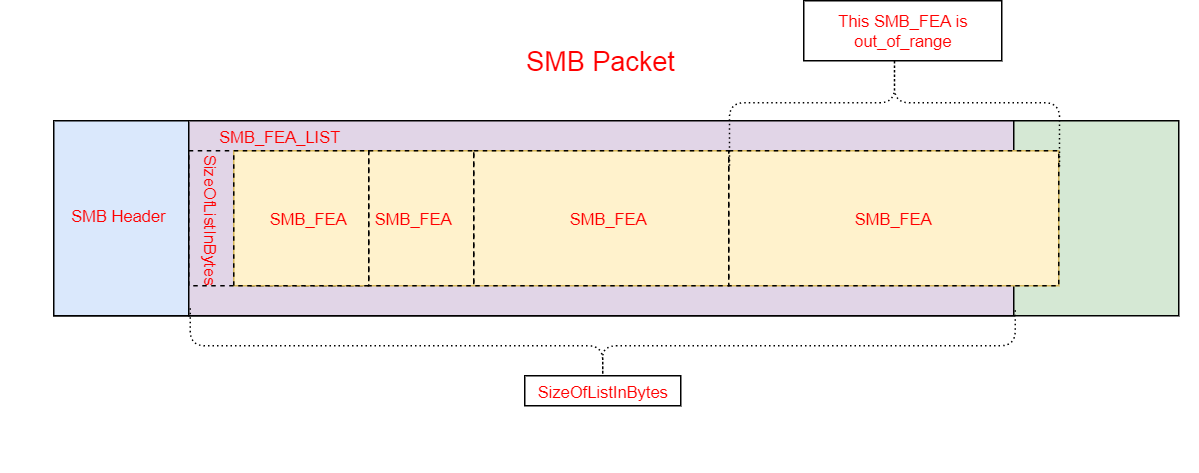
\includegraphics[width=15cm]{checkpoint_before_shrink.png}
    \caption[FEAList vor Verkleinerung, Nadav Grossmann (Checkpoint Research), URL. <https://research.checkpoint.com/wp-content/uploads/2017/09/eternalblue4.png>]{Speicherbelegung der FEA Liste vor Verkleinerung}
    \label{img:fealist_before_shrinking}
\end{figure}

\noindent
SizeOfListInBytes ist eine Membervariable in DWORD-Größe, wird aber im Falle eines ungültigen FEA lediglich als Variable in WORD-größe behandelt, weshalb die zwei most significant Bytes nicht verändert werden. Das sorgt dafür, dass im Falle eines Wertes mit Bytegröße über 216 die SizeOfListInBytes vergrößert und nicht verkleinert wird. Hierdurch wird weniger Speicher reserviert, als nach Konvertierung der Liste benötigt wird, es kommt also zu einem out-of-bound-write im Arbeitsspeicher.

\begin{figure}[H]
    \centering
    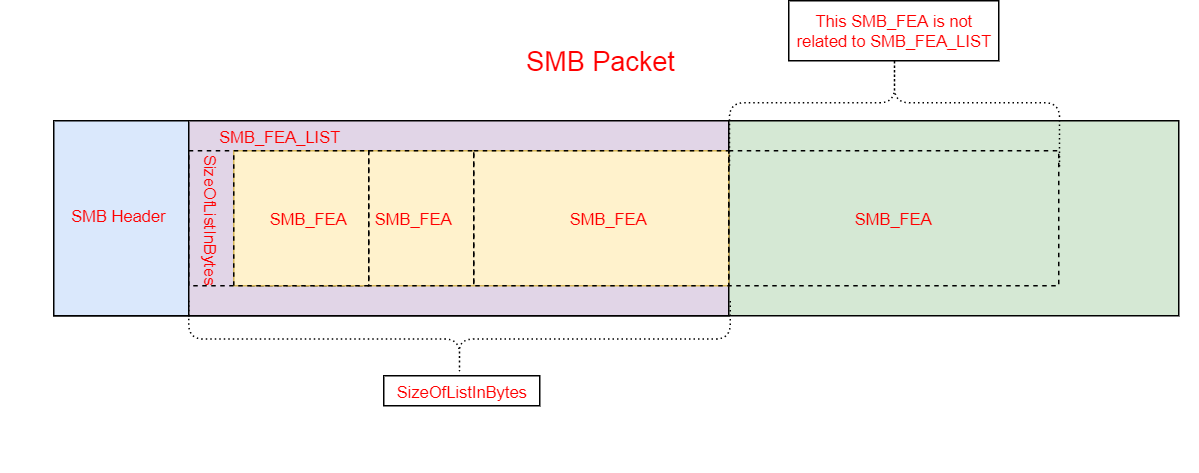
\includegraphics[width=15cm]{checkpoint_after_shrink_correct.png}
    \caption[FEAList nach korrekter Verkleinerung, Nadav Grossmann (Checkpoint Research). URL: <https://research.checkpoint.com/wp-content/uploads/2017/09/eternalblue5.png>]{Speicherbelegung der FEA Liste nach korrekter Verkleinerung}
    \label{img:fealist_after_shrinking_correctly}
\end{figure}

\begin{figure}[H]
    \centering
    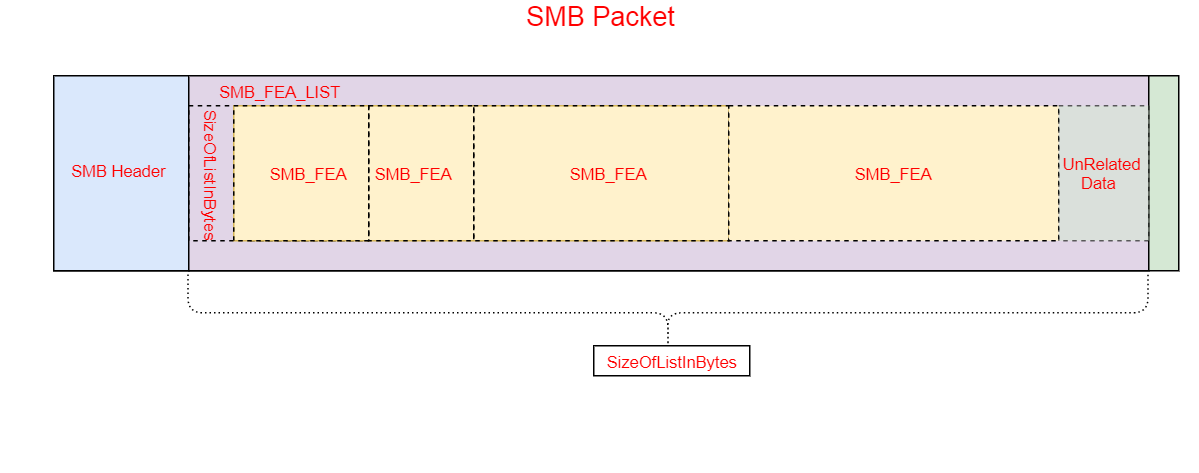
\includegraphics[width=15cm]{checkpoint_after_shrink_error.png}
    \caption[FEAList nach fehlerhafter Verkleinerung, Nadav Grossmann (Checkpoint Research). URL: <https://research.checkpoint.com/wp-content/uploads/2017/09/eternalblue6.png>]{Speicherbelegung der FEA Liste nach fehlerhafter Verkleinerung}
    \label{img:fealist_after_shrinking_incorrectly}
\end{figure}

\section{Falsches Parsen des SMB Datensegments}
Für die Übertragung von Daten kommen zwei SMB Commands und deren Subcommands zum Einsatz, die für die Übertragung von Daten verantwortlich sind: \verb|SMB_COM_TRANSACTION2| und \verb|SMB_COM_NT_TRANSACT|. Durch Anhängen von \verb|_SECOND| kann jeweils der sekundäre Befehl gebildet werden. Ist die in der Variable \verb|total_data_to_send| zu übertragende Datenmenge größer als die maximale Buffergröße, so werden die im primären Befehl noch ausstehenden Daten aufgeteilt und nach dem initialen Paket mittels des mit \verb|_SECONDARY|  gebildeten Commands versendet, bis die zu übermittelnden Daten vollständig sind.

\noindent
Die zwei Befehle samt deren Subcommands unterscheiden sich nur gering, aber in einem für den Exploit essentiellen Punkt signifikant, was für den erfolgreichen Hack von Bedeutung ist. Während \verb|SMB_COM_TRANSACTION2| die Bytegröße der zu sendenden Daten in einem Header Parameter in WORD-Größe abspeichert, nutzt \verb|SMB_COM_NT_TRANSACTION| hierfür einen in DWORD-Größe.

\noindent
Ein weiterer wichtiger Faktor ist auch, dass nicht geprüft wird, mit welchem der beiden Befehle eine Transaktion gestartet wurde. Dieser Unterschied in der maximal adressierbaren Datenmenge der Transaktionsbefehlstypen und der Mangel an Validierung, ob die Transaktionsart gleich bleibt, lassen sich für einen Angreifer ausnutzen, indem auf \verb|SMB_COM_NT_TRANSACT_SECONDARY| ein \verb|SMB_COM_TRANSACTION2| gesendet wird. Das wiederum kann zum Parsen der falschen Daten führen. Dies ermöglicht den das fehlerhafte Parsen der Daten durch behandeln des WORD-großen Header Parameters in \verb|_TRANSACTION2| als DWORD, was die FEAs malformed und somit ungültig werden lässt.

\section{Allokation von Speicher im Non-Paged Memory Pool}
Um eine Session beim Server über Port 445 aufbauen zu können, wird ein Authentifikationsrequest über die Funktion \verb|SMB_COM_SESSION_SETUP_ANDX| gesendet, was den User Logon beim Server etabliert und eine UID kreiert. Auch beim Anmelden gibt es wieder zwei unterschiedliche Formate, namentlich LM/NTLM und NTLMv2, auch bekannt als NTLM SSP. Diese besitzen bei eine ähnliche zweiteilige Struktur, welche aus zwei Blöcken, \verb|SMB_Parameters| und \verb|SMB_Data|, besteht.
\verb|SMB_Parameters| speichert in sich mehrere Parameter, die jeweils maximal vier Bytes an Speicher einnehmen können. Auch ist hier die Variable WordCount zu finden, welche die Länge der \verb|SMB_Parameters| Daten in WORDs angibt. Anhand von WordCount kann in der Regel auch der Typ der Struktur erkannt werden, da dieser bei LM und NTLM stets 13 und bei NTLMv2 12 beträgt, was für das Gelingen des Exploits von großer Bedeutung ist.
Der zweite Teil beider Formate, \verb|SMB_Data|, beinhaltet Daten in unterschiedlicher Größe, wobei eine Variable namens ByteCount den benötigten Speicherplatz festhält. In beiden Fällen führt der Server einen Integritätscheck mit einer Funktion namens SrvValidateSmb aus, um zu überprüfen, ob die Struktur eingehalten und unbeschädigt ist.

\chapter{Prävention und Schutz}
Wie bei den meisten anderen Softwareprobleme empfielt sich, regelmäßig Updates aufzuspielen, um Sicherheitslücken durch Patches zu schließen. Das Update, das Hacking mittels des EternalBlue Exploits verhindert, ist seit März 2017 für alle relevanten Windows Produkte verfügbar.
Um zu überprüfen, ob eine Maschine die Sicherheitslücke noch aufweist, hat die Firma Sophos ein Powershell-Skript bereit gestellt, welches auf Windowsversion, Betriebssystem und Updates prüft \cite{SAV}.
Neuere Windows 10 und Windows Server Installationen werden ab dem Fall Creators Update 2017 auch nicht mehr standardmäßig die seit 2014 offiziell als veraltet geltende SMBv1 Schnittstelle installiert haben. Sollte das Protokoll für Legacy Geräte noch benötigt werden, kann es aber jederzeit über die Windows-Features wieder installiert werden \cite{MS:Fix}.
Da das SMBv1-Protokoll als relativ unsicher gilt und hauptsächlich für die Unterstützung alter Systeme benötigt wird, kann es auf den meisten Rechnern ohne negative Folgen deaktiviert bzw. deinstalliert werden \cite{WP}. Das kann zum Beispiel unter Windows 10 über die Funktion "Windows-Features" der Systemsteuerung gemacht werden.

\clearpage
\label{sec:literatur}
\renewcommand{\bibname}{Quellenverzeichnis}
\bibliographystyle{unsrtdin}
\bibliography{itsec}
\addcontentsline{toc}{chapter}{Quellen- und Literaturverzeichnis}

\end{document}